%----------------------------------------------------------------------------------------
%	CHAPTER - RESEARCH METHOD
%----------------------------------------------------------------------------------------

\chapter{Research Method} % Main chapter title

\label{Research Method} % Change X to a consecutive number; for referencing this chapter elsewhere, use \ref{ChapterX}

%----------------------------------------------------------------------------------------
%	SECTION 1
%----------------------------------------------------------------------------------------

\section{Introduction}

In this chapter, the research methodology of this thesis is described. An interpretive research philosophy is assumed for this thesis. \cite{Hevner2010} defined different research strategies out of which design science is applied.


%----------------------------------------------------------------------------------------
%	SECTION 2
%----------------------------------------------------------------------------------------

\section{Philosophy}

The research philosophy shows how the researcher views the world and the knowledge that has to be developed as well as its nature.

\cite{Saunders2009} defines four different research philosophies:
\begin{itemize}[noitemsep,nolistsep]
	\item Positivism \textit{(only observable phenomena will lead
		to the production of credible data)}
	\item Realism \textit{(do objects exist independently of our
		knowledge of their existence?)}
	\item Interpretivism \textit{(understanding differences 
		between humans as social actors)}
	\item Pragmatism \textit{(do you have to adopt one position?)}
\end{itemize}

In addition, \cite{Saunders2009} also lists three major ways of how to think about the different research philosophies:
\begin{itemize}[noitemsep,nolistsep]
	\item Epistemology \textit{(the view of the nature of reality or being)}
	\item Ontology \textit{(the view of what constitutes acceptable knowledge)}
	\item Axiology \textit{(the view of the role of values in research)}
\end{itemize}

% TODO: check for Vaishnavi reference
An interpretive research philosophy, as defined by \cite{Vaishnavi2008} and \cite{Saunders2009}, is assumed for this thesis since it has the biggest match out of all possible philosophies. The reason for this can be found upon evaluating the different views. \newline
Gesture controllers and 360° motion tracking provide, from a technical point of view, a standard input device. What individuals actors do with the available means however is completely subjective. From an \textbf{epistemology view}, the researcher interprets the presented situation and his actions are motivated based on how he percepts the details of this situation. \newline
In the \textbf{ontology view}, the researcher's view of the nature of reality is socially constructed, subjective and may change. In virtual reality, everything depends on how he perceives and interprets the visualizations; every individual has a different view of the reality. \newline
From the \textbf{axiology view}, the view of what role the values play, the researcher is part of what is being researched as he decides on his own how to interact with the virtual reality and what usable gestures are defined. This is subjective as it cannot be separated from the research and thus there will be not the one solution, but merely one out of many. \newline
Finally, looking at the data collection methods, only small samples of sensor data from gesture controllers and 360° motion tracking will be collected. This data can be investigated quantitative (is the gesture effective in its purpose?), qualitative (does the gesture what I intended to do?) or also in combination


%----------------------------------------------------------------------------------------
%	SECTION 3
%----------------------------------------------------------------------------------------

\section{Approach}

Based on \cite{Saunders2009}, a research approach can either be deductive (testing a theory), inductive (building a theory) or a combination of them. Table \ref{tbl:inductivedeductive} shows the major differences between deductive and inductive approach.
\begin{table}[h!]
	\begin{center}
		\begin{tabular}{ p{6.5cm} p{7.5cm} }
			\toprule
			\textbf{Deduction emphasises} & \textbf{Induction emphasises} \\
			\midrule
			scientific principles & less concern with the need to generalise \\
			moving from theory to data & a close understanding of the research context  \\
			the need to explain causal relationships between variables & gaining an understanding of the meanings humans attach to events \\
			the collection of quantitative data & the collection of qualitative data \\
			the application of controls to ensure validity of data & a more flexible structure to permit changes of research emphasis as the research progresses \\
			the operationalisation of concepts to ensure clarity of definition & a realisation that the researcher is part of the research process \\
			a highly structured approach & \\
			researcher independence of what is being researched & \\
			the necessity to select samples of sufficient size in order to generalise conclusions & \\
			\bottomrule
		\end{tabular}
		\caption[Major differences between deductive and inductive approaches to research]{Major differences between deductive and inductive approaches to research (adopted from {\citealp[pg. 127]{Saunders2009}})}
		\label{tbl:inductivedeductive}
	\end{center}
\end{table}
\newline
With literature review, knowledge about the current state of interaction possibilities with virtual reality is collected and analysed. Based on the gained information and a close understanding of the research context, a theory can be formulated. With the help of a to be built prototype this theory can be evaluated and tested by the researcher. This is a typical procedure of an inductive approach as described by \cite{Saunders2009}. \newline
The deductive approach starts at the other end as first the theory is built by searching to explain causal relationships between variables. The test of this theory requires the collection of quantitative data which does not match the goal of this thesis, since its focus is more theoretical. \newline
\cite{Creswell2014} further defined a set of criteria for selecting a research approach based on the situation of current research. If only little research has been done yet and the topic first has to be explored and understood, then a qualitative (inductive) approach suits the best \citep[pg 50]{Creswell2014}. Although virtual reality in itself has been researched for quite a while, it indeed is quite new to have gesture controllers and 360° motion tracking available as well. This makes the thesis a good match for an inductive approach.


%----------------------------------------------------------------------------------------
%	SECTION 4
%----------------------------------------------------------------------------------------

\section{Strategy}

%-----------------------------------
%	SUBSECTION 1
%-----------------------------------

\subsection{Introduction}

\cite{Saunders2009} consider seven different research strategies:
\begin{itemize}[noitemsep,nolistsep]
	\item Experiment \textit{(study causal links)}
	\item Survey \textit{(answering who, what, where, how much and how many questions)}
	\item Case Study \textit{(empirical investigation within its real life context)}
	\item Action Research \textit{(explicit focus on research in action)}
	\item Grounded Theory \textit{(emphasis upon developing and building a theory)}
	\item Ethnography \textit{(describe and explain the social world the research subjects inhabit)}
	\item Archival Research \textit{(administrative records and documents as principle data source)}
\end{itemize}
In Information Systems, \cite{Hevner2010} suggest \textbf{design science} as another research strategy which inherently is a problem solving process. For this strategy, seven guidelines for design science research are derived which can be summarized in two main characteristics \citep{Hevner2010}: On the one hand the creation of an innovative, purposeful artefact for a specified problem domain, and on the other hand the thorough evaluation of the artefact and its highly applicable in practice. Both of them are considered crucial for this thesis. \newline
The artefact is represented by the prototype of a virtual reality application that utilizes the additional sensor information from gesture controllers and 360° motion tracking. The relevance for practice and its applicability is given by feasible enhancements to existing solutions that are already used in practice.



%-----------------------------------
%	SUBSECTION 2
%-----------------------------------

\subsection{Design Research Cycle}

\cite{Vaishnavi2008} and \cite{Hevner2010} define \gls{dsr} as a research paradigm in which questions that are relevant to human problems are answered with the creation of innovative artefacts. As an approach for conducting design science research, \cite{Vaishnavi2004} defined a design science research process model (\gls{dsr} Cycle). This cycle follows a step-wise approach and has been structured in the five phases that are as follows: awareness of the problem, suggestion, development, evaluation and conclusion (Figure \ref{fig:dsrcycle}). In the following chapters, these five phases and their relation to this thesis are discussed.
\newline
%    h (here) - same location
%    t (top) - top of page
%    b (bottom) - bottom of page
%    p (page) - on an extra page
%    ! (override) - will force the specified location
\begin{figure}[h]
	\begin{center}
		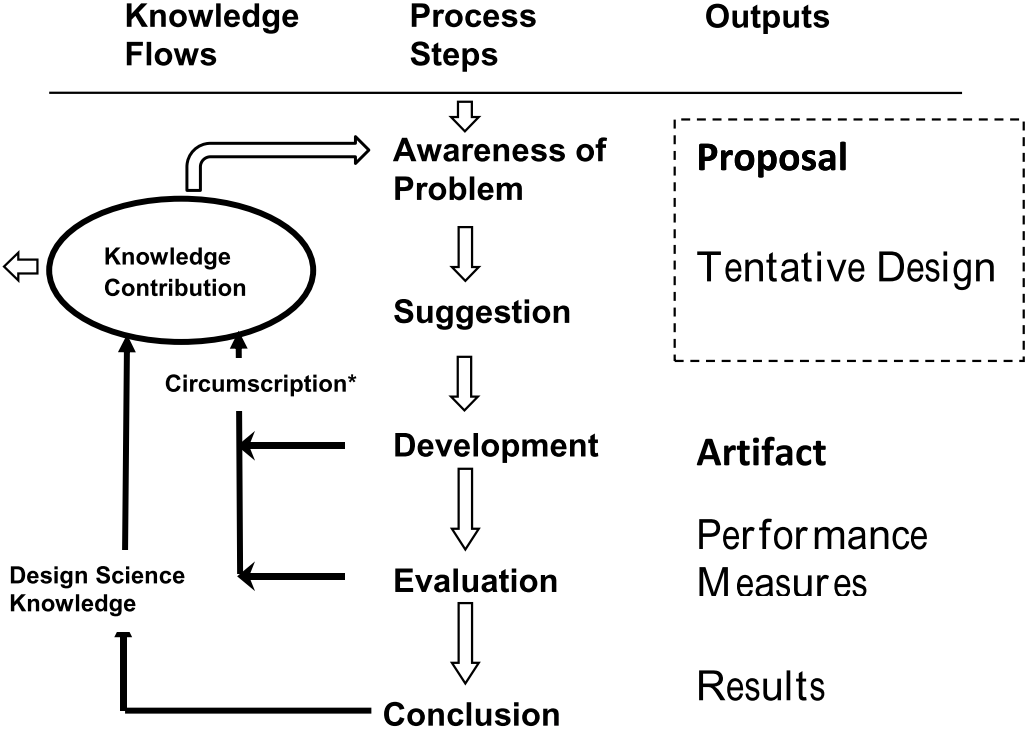
\includegraphics[width=11cm]{03_Figures/02_DSR_Cycle/DSR_Cycle.png}
		\caption[Design Science Research Process Model (DSR Cycle)]{Design Science Research Process Model (DSR Cycle) \citep{Vaishnavi2004}}
		\label{fig:dsrcycle}
	\end{center}
\end{figure}


%-----------------------------------
%	SUBSUBSECTION 1
%-----------------------------------

\subsubsection{Awareness}

\cite{Hevner2010} defined in the initial step of the \gls{dsr} Cycle the awareness of the problem, where
\begin{itemize}[noitemsep,nolistsep]
	\item the problem is identified.
	\item the problem is defined.
	\item the value of a solution is justified.
\end{itemize}
This is the foundation of all subsequent steps as the suggestion, development and evaluation phases all focus on the identified problem. \newline
In this thesis, the identification and definition of the problem is covered in chapter \ref{ChapterIntroduction} (introduction) whereas the justification of the value of a solution is established in the literature of chapter \ref{ChapterLiteratureReview} in the form of research gaps.
The literature review shows that while there has been research done on the interaction patterns for \textit{Travel} and \textit{Selection}, the \textit{Motivation} is only covered on the surface. Furthermore, although guidelines for the interaction patterns are available, there are no practical suggestions/recommendations on how this could look like in practice or whether these guidelines really make sense once applied. The motivation for an improvement lies in the importance of \textit{Manipulation} patterns or uses in practice and recommendations on how matching interactions patterns have to be designed with the corresponding method in mind.


%-----------------------------------
%	SUBSUBSECTION 2
%-----------------------------------

\subsubsection{Suggestion}

blub


%-----------------------------------
%	SUBSUBSECTION 3
%-----------------------------------

\subsubsection{Development}

In the development phase, the existing knowledge together with the defined problem definition is synthesized into an artefact that solves the mentioned problem \citep{Vaishnavi2008}. In this thesis, the artefact is the virtual reality prototype application.


%-----------------------------------
%	SUBSUBSECTION 4
%-----------------------------------

\subsubsection{Evaluation}

In order to demonstrate that with the proposed solution the problem can be solved, \cite{Hevner2010}  defined that the artefacts needs to be evaluated.
Table XXX shows possible evaluation methods for designed artefacts  that are based on \cite{Hevner2004}. For this research, the methods from \textit{Testing} and \textit{Descriptive} will be applied.


\begin{table}[h]
	\begin{center}
		\begin{tabular}{ | m{4cm} | p{10cm} | } 
			\hline
			\multirow{2}{*}{1. Observational} &
				Case Study: Study artefact in depth in business environment \\
				\cline{2-2}
				& Field Study: Monitor use of artefact in multiple projects \\
			\hline
			\multirow{4}{*}{2. Analytical} &
				Static Analysis: Examine structure of artefact for static qualities (e.g., complexity) \\
				\cline{2-2}
				& Architecture Analysis: Study fit of artefact into technical IS architecture \\
				\cline{2-2}
				& Optimization: Demonstrate inherent optimal properties of artefact or provide optimality bounds on artefact behaviour \\
				\cline{2-2}
				& Dynamic Analysis: Study artefact in use for dynamic qualities (e.g., performance) \\
			\hline
			\multirow{2}{*}{3. Experimental} &
				Controlled Experiment: Study artefact in controlled environment for qualities (e.g., usability) \\
				\cline{2-2}
				& Simulation - Execute artefact with artificial data \\
			\hline
			\multirow{2}{*}{4. Testing} &
				\cellcolor{green!25}Functional (Black Box) Testing:  Execute artefact interfaces to discover failures and identify defects \\
				\hhline{|~|-|}
				& \cellcolor{green!25}Structural (White Box) Testing:  Perform coverage testing of some metric (e.g. execution paths) in the artefact implementation \\
			\hline
			\multirow{2}{*}{5. Descriptive} &
				\cellcolor{green!25}Informed Argument:  Use information from the knowledge base (e.g. relevant research) to build a convincing argument for the artefact's utility \\
				\hhline{|~|-|}
				& \cellcolor{green!25}Scenarios: Construct detailed scenarios around the artefact to demonstrate its utility \\
			\hline
		\end{tabular}
		\caption[Design Evaluation Methods]{Design Evaluation Methods (based on \cite{Hevner2004})}
		\label{tbl:designevaluationmethods}
	\end{center}
\end{table}


%-----------------------------------
%	SUBSUBSECTION 5
%-----------------------------------

\subsubsection{Conclusion}

blub


%----------------------------------------------------------------------------------------
%	SECTION 5
%----------------------------------------------------------------------------------------

\section{Timeline}

As part of the master thesis research proposal, the literature review is conducted alongside its analysis. The development and evaluation of the prototype as part of the design science research will be done in the implementation phase of the master thesis.


%----------------------------------------------------------------------------------------
%	SECTION 6
%----------------------------------------------------------------------------------------

\section{Data collection}

Quantitative vs Qualitative

--> check The research choice defines how data is collected or analysed. This can be either in a quantitative way (numerical data) – qualitative way (non-numerical) – or mixed (Saunders et al., 2009).

%----------------------------------------------------------------------------------------
%	SECTION 7
%----------------------------------------------------------------------------------------

% \section{Data analysis}


%----------------------------------------------------------------------------------------
%	SECTION 8
%----------------------------------------------------------------------------------------

\section{Conclusion}

blub

